\PassOptionsToPackage{unicode=true}{hyperref} % options for packages loaded elsewhere
\PassOptionsToPackage{hyphens}{url}
%
\documentclass[]{article}
\usepackage{lmodern}
\usepackage{amssymb,amsmath}
\usepackage{ifxetex,ifluatex}
\usepackage{fixltx2e} % provides \textsubscript
\ifnum 0\ifxetex 1\fi\ifluatex 1\fi=0 % if pdftex
  \usepackage[T1]{fontenc}
  \usepackage[utf8]{inputenc}
  \usepackage{textcomp} % provides euro and other symbols
\else % if luatex or xelatex
  \usepackage{unicode-math}
  \defaultfontfeatures{Ligatures=TeX,Scale=MatchLowercase}
\fi
% use upquote if available, for straight quotes in verbatim environments
\IfFileExists{upquote.sty}{\usepackage{upquote}}{}
% use microtype if available
\IfFileExists{microtype.sty}{%
\usepackage[]{microtype}
\UseMicrotypeSet[protrusion]{basicmath} % disable protrusion for tt fonts
}{}
\IfFileExists{parskip.sty}{%
\usepackage{parskip}
}{% else
\setlength{\parindent}{0pt}
\setlength{\parskip}{6pt plus 2pt minus 1pt}
}
\usepackage{hyperref}
\hypersetup{
            pdftitle={2020-01-05},
            pdfborder={0 0 0},
            breaklinks=true}
\urlstyle{same}  % don't use monospace font for urls
\usepackage[margin=1in]{geometry}
\usepackage{color}
\usepackage{fancyvrb}
\newcommand{\VerbBar}{|}
\newcommand{\VERB}{\Verb[commandchars=\\\{\}]}
\DefineVerbatimEnvironment{Highlighting}{Verbatim}{commandchars=\\\{\}}
% Add ',fontsize=\small' for more characters per line
\usepackage{framed}
\definecolor{shadecolor}{RGB}{248,248,248}
\newenvironment{Shaded}{\begin{snugshade}}{\end{snugshade}}
\newcommand{\AlertTok}[1]{\textcolor[rgb]{0.94,0.16,0.16}{#1}}
\newcommand{\AnnotationTok}[1]{\textcolor[rgb]{0.56,0.35,0.01}{\textbf{\textit{#1}}}}
\newcommand{\AttributeTok}[1]{\textcolor[rgb]{0.77,0.63,0.00}{#1}}
\newcommand{\BaseNTok}[1]{\textcolor[rgb]{0.00,0.00,0.81}{#1}}
\newcommand{\BuiltInTok}[1]{#1}
\newcommand{\CharTok}[1]{\textcolor[rgb]{0.31,0.60,0.02}{#1}}
\newcommand{\CommentTok}[1]{\textcolor[rgb]{0.56,0.35,0.01}{\textit{#1}}}
\newcommand{\CommentVarTok}[1]{\textcolor[rgb]{0.56,0.35,0.01}{\textbf{\textit{#1}}}}
\newcommand{\ConstantTok}[1]{\textcolor[rgb]{0.00,0.00,0.00}{#1}}
\newcommand{\ControlFlowTok}[1]{\textcolor[rgb]{0.13,0.29,0.53}{\textbf{#1}}}
\newcommand{\DataTypeTok}[1]{\textcolor[rgb]{0.13,0.29,0.53}{#1}}
\newcommand{\DecValTok}[1]{\textcolor[rgb]{0.00,0.00,0.81}{#1}}
\newcommand{\DocumentationTok}[1]{\textcolor[rgb]{0.56,0.35,0.01}{\textbf{\textit{#1}}}}
\newcommand{\ErrorTok}[1]{\textcolor[rgb]{0.64,0.00,0.00}{\textbf{#1}}}
\newcommand{\ExtensionTok}[1]{#1}
\newcommand{\FloatTok}[1]{\textcolor[rgb]{0.00,0.00,0.81}{#1}}
\newcommand{\FunctionTok}[1]{\textcolor[rgb]{0.00,0.00,0.00}{#1}}
\newcommand{\ImportTok}[1]{#1}
\newcommand{\InformationTok}[1]{\textcolor[rgb]{0.56,0.35,0.01}{\textbf{\textit{#1}}}}
\newcommand{\KeywordTok}[1]{\textcolor[rgb]{0.13,0.29,0.53}{\textbf{#1}}}
\newcommand{\NormalTok}[1]{#1}
\newcommand{\OperatorTok}[1]{\textcolor[rgb]{0.81,0.36,0.00}{\textbf{#1}}}
\newcommand{\OtherTok}[1]{\textcolor[rgb]{0.56,0.35,0.01}{#1}}
\newcommand{\PreprocessorTok}[1]{\textcolor[rgb]{0.56,0.35,0.01}{\textit{#1}}}
\newcommand{\RegionMarkerTok}[1]{#1}
\newcommand{\SpecialCharTok}[1]{\textcolor[rgb]{0.00,0.00,0.00}{#1}}
\newcommand{\SpecialStringTok}[1]{\textcolor[rgb]{0.31,0.60,0.02}{#1}}
\newcommand{\StringTok}[1]{\textcolor[rgb]{0.31,0.60,0.02}{#1}}
\newcommand{\VariableTok}[1]{\textcolor[rgb]{0.00,0.00,0.00}{#1}}
\newcommand{\VerbatimStringTok}[1]{\textcolor[rgb]{0.31,0.60,0.02}{#1}}
\newcommand{\WarningTok}[1]{\textcolor[rgb]{0.56,0.35,0.01}{\textbf{\textit{#1}}}}
\usepackage{graphicx,grffile}
\makeatletter
\def\maxwidth{\ifdim\Gin@nat@width>\linewidth\linewidth\else\Gin@nat@width\fi}
\def\maxheight{\ifdim\Gin@nat@height>\textheight\textheight\else\Gin@nat@height\fi}
\makeatother
% Scale images if necessary, so that they will not overflow the page
% margins by default, and it is still possible to overwrite the defaults
% using explicit options in \includegraphics[width, height, ...]{}
\setkeys{Gin}{width=\maxwidth,height=\maxheight,keepaspectratio}
\setlength{\emergencystretch}{3em}  % prevent overfull lines
\providecommand{\tightlist}{%
  \setlength{\itemsep}{0pt}\setlength{\parskip}{0pt}}
\setcounter{secnumdepth}{0}
% Redefines (sub)paragraphs to behave more like sections
\ifx\paragraph\undefined\else
\let\oldparagraph\paragraph
\renewcommand{\paragraph}[1]{\oldparagraph{#1}\mbox{}}
\fi
\ifx\subparagraph\undefined\else
\let\oldsubparagraph\subparagraph
\renewcommand{\subparagraph}[1]{\oldsubparagraph{#1}\mbox{}}
\fi

% set default figure placement to htbp
\makeatletter
\def\fps@figure{htbp}
\makeatother


\title{2020-01-05}
\author{}
\date{\vspace{-2.5em}2021-01-05}

\begin{document}
\maketitle

\hypertarget{tidytuesday}{%
\section{TidyTuesday}\label{tidytuesday}}

Join the R4DS Online Learning Community in the weekly \#TidyTuesday
event! Every week we post a raw dataset, a chart or article related to
that dataset, and ask you to explore the data. While the dataset will be
``tamed'', it will not always be tidy! As such you might need to apply
various R for Data Science techniques to wrangle the data into a true
tidy format. The goal of TidyTuesday is to apply your R skills, get
feedback, explore other's work, and connect with the greater \#RStats
community! As such we encourage everyone of all skills to participate!

\begin{Shaded}
\begin{Highlighting}[]
\KeywordTok{library}\NormalTok{(tidyverse)}
\end{Highlighting}
\end{Shaded}

\begin{verbatim}
## -- Attaching packages --------------------------- tidyverse 1.3.0 --
\end{verbatim}

\begin{verbatim}
## v ggplot2 3.3.2     v purrr   0.3.3
## v tibble  2.1.3     v dplyr   0.8.4
## v tidyr   1.0.2     v stringr 1.4.0
## v readr   1.3.1     v forcats 0.4.0
\end{verbatim}

\begin{verbatim}
## Warning: package 'ggplot2' was built under R version 3.6.2
\end{verbatim}

\begin{verbatim}
## -- Conflicts ------------------------------ tidyverse_conflicts() --
## x dplyr::filter() masks stats::filter()
## x dplyr::lag()    masks stats::lag()
\end{verbatim}

\begin{Shaded}
\begin{Highlighting}[]
\KeywordTok{library}\NormalTok{(tidytuesdayR)}
\end{Highlighting}
\end{Shaded}

\begin{verbatim}
## Warning: package 'tidytuesdayR' was built under R version 3.6.2
\end{verbatim}

\begin{Shaded}
\begin{Highlighting}[]
\KeywordTok{library}\NormalTok{(lubridate)}
\end{Highlighting}
\end{Shaded}

\begin{verbatim}
## 
## Attaching package: 'lubridate'
\end{verbatim}

\begin{verbatim}
## The following object is masked from 'package:base':
## 
##     date
\end{verbatim}

\begin{Shaded}
\begin{Highlighting}[]
\KeywordTok{library}\NormalTok{(dplyr)}
\KeywordTok{library}\NormalTok{(tidyr)}
\CommentTok{#install.packages("countrycode")}
\end{Highlighting}
\end{Shaded}

\hypertarget{load-the-weekly-data}{%
\section{Load the weekly Data}\label{load-the-weekly-data}}

Dowload the weekly data and make available in the \texttt{tt} object.

\begin{Shaded}
\begin{Highlighting}[]
\CommentTok{# download the data}
\NormalTok{tt <-}\StringTok{ }\KeywordTok{tt_load}\NormalTok{(}\StringTok{"2021-01-05"}\NormalTok{)}
\end{Highlighting}
\end{Shaded}

\begin{verbatim}
## --- Compiling #TidyTuesday Information for 2021-01-05 ----
\end{verbatim}

\begin{verbatim}
## --- There is 1 file available ---
\end{verbatim}

\begin{verbatim}
## --- Starting Download ---
\end{verbatim}

\begin{verbatim}
## 
##  Downloading file 1 of 1: `transit_cost.csv`
\end{verbatim}

\begin{verbatim}
## --- Download complete ---
\end{verbatim}

\begin{Shaded}
\begin{Highlighting}[]
\CommentTok{#saving the data as a variable}
\NormalTok{transit <-}\StringTok{ }\NormalTok{tt}\OperatorTok{$}\StringTok{'transit_cost'}
\end{Highlighting}
\end{Shaded}

\hypertarget{readme}{%
\section{Readme}\label{readme}}

Take a look at the readme for the weekly data to get insight on the
dataset. This includes a data dictionary, source, and a link to an
article on the data.

\begin{Shaded}
\begin{Highlighting}[]
\KeywordTok{readme}\NormalTok{(tt)}
\KeywordTok{print}\NormalTok{(tt)}
\end{Highlighting}
\end{Shaded}

\hypertarget{glimpse-data}{%
\section{Glimpse Data}\label{glimpse-data}}

Take an initial look at the format of the data available.

\begin{Shaded}
\begin{Highlighting}[]
\NormalTok{tt }\OperatorTok\StringTok{ }
\StringTok{  }\KeywordTok{map}\NormalTok{(glimpse)}
\end{Highlighting}
\end{Shaded}

\begin{verbatim}
## Observations: 544
## Variables: 20
## $ e                <dbl> 7136, 7137, 7138, 7139, 7144, 7145, 7146, 7147, 71...
## $ country          <chr> "CA", "CA", "CA", "CA", "CA", "NL", "CA", "US", "U...
## $ city             <chr> "Vancouver", "Toronto", "Toronto", "Toronto", "Tor...
## $ line             <chr> "Broadway", "Vaughan", "Scarborough", "Ontario", "...
## $ start_year       <chr> "2020", "2009", "2020", "2020", "2020", "2003", "2...
## $ end_year         <chr> "2025", "2017", "2030", "2030", "2030", "2018", "2...
## $ rr               <dbl> 0, 0, 0, 0, 0, 0, 0, 0, 0, 0, 0, 0, 0, 0, 0, 0, 0,...
## $ length           <dbl> 5.7, 8.6, 7.8, 15.5, 7.4, 9.7, 5.8, 5.1, 4.2, 4.2,...
## $ tunnel_per       <chr> "87.72%", "100.00%", "100.00%", "57.00%", "100.00%...
## $ tunnel           <dbl> 5.0, 8.6, 7.8, 8.8, 7.4, 7.1, 5.8, 5.1, 4.2, 4.2, ...
## $ stations         <dbl> 6, 6, 3, 15, 6, 8, 5, 2, 2, 2, 3, 3, 4, 7, 13, 4, ...
## $ source1          <chr> "Plan", "Media", "Wiki", "Plan", "Plan", "Wiki", "...
## $ cost             <dbl> 2830, 3200, 5500, 8573, 5600, 3100, 4500, 1756, 36...
## $ currency         <chr> "CAD", "CAD", "CAD", "CAD", "CAD", "EUR", "CAD", "...
## $ year             <dbl> 2018, 2013, 2018, 2019, 2020, 2009, 2018, 2012, 20...
## $ ppp_rate         <dbl> 0.840, 0.810, 0.840, 0.840, 0.840, 1.300, 0.840, 1...
## $ real_cost        <chr> "2377.2", "2592", "4620", "7201.32", "4704", "4030...
## $ cost_km_millions <dbl> 417.05263, 301.39535, 592.30769, 464.60129, 635.67...
## $ source2          <chr> "Media", "Media", "Media", "Plan", "Media", "Media...
## $ reference        <chr> "https://www.translink.ca/Plans-and-Projects/Rapid...
\end{verbatim}

\begin{verbatim}
## $transit_cost
## # A tibble: 544 x 20
##        e country city  line  start_year end_year    rr length tunnel_per tunnel
##    <dbl> <chr>   <chr> <chr> <chr>      <chr>    <dbl>  <dbl> <chr>       <dbl>
##  1  7136 CA      Vanc~ Broa~ 2020       2025         0    5.7 87.72%        5  
##  2  7137 CA      Toro~ Vaug~ 2009       2017         0    8.6 100.00%       8.6
##  3  7138 CA      Toro~ Scar~ 2020       2030         0    7.8 100.00%       7.8
##  4  7139 CA      Toro~ Onta~ 2020       2030         0   15.5 57.00%        8.8
##  5  7144 CA      Toro~ Yong~ 2020       2030         0    7.4 100.00%       7.4
##  6  7145 NL      Amst~ Nort~ 2003       2018         0    9.7 73.00%        7.1
##  7  7146 CA      Mont~ Blue~ 2020       2026         0    5.8 100.00%       5.8
##  8  7147 US      Seat~ U-Li~ 2009       2016         0    5.1 100.00%       5.1
##  9  7152 US      Los ~ Purp~ 2020       2027         0    4.2 100.00%       4.2
## 10  7153 US      Los ~ Purp~ 2018       2026         0    4.2 100.00%       4.2
## # ... with 534 more rows, and 10 more variables: stations <dbl>, source1 <chr>,
## #   cost <dbl>, currency <chr>, year <dbl>, ppp_rate <dbl>, real_cost <chr>,
## #   cost_km_millions <dbl>, source2 <chr>, reference <chr>
\end{verbatim}

\begin{Shaded}
\begin{Highlighting}[]
\KeywordTok{head}\NormalTok{(transit)}
\end{Highlighting}
\end{Shaded}

\begin{verbatim}
## # A tibble: 6 x 20
##       e country city  line  start_year end_year    rr length tunnel_per tunnel
##   <dbl> <chr>   <chr> <chr> <chr>      <chr>    <dbl>  <dbl> <chr>       <dbl>
## 1  7136 CA      Vanc~ Broa~ 2020       2025         0    5.7 87.72%        5  
## 2  7137 CA      Toro~ Vaug~ 2009       2017         0    8.6 100.00%       8.6
## 3  7138 CA      Toro~ Scar~ 2020       2030         0    7.8 100.00%       7.8
## 4  7139 CA      Toro~ Onta~ 2020       2030         0   15.5 57.00%        8.8
## 5  7144 CA      Toro~ Yong~ 2020       2030         0    7.4 100.00%       7.4
## 6  7145 NL      Amst~ Nort~ 2003       2018         0    9.7 73.00%        7.1
## # ... with 10 more variables: stations <dbl>, source1 <chr>, cost <dbl>,
## #   currency <chr>, year <dbl>, ppp_rate <dbl>, real_cost <chr>,
## #   cost_km_millions <dbl>, source2 <chr>, reference <chr>
\end{verbatim}

\hypertarget{wrangle}{%
\section{Wrangle}\label{wrangle}}

Explore the data and process it into a nice format for plotting! Access
each dataset by name by using a dollarsign after the \texttt{tt} object
and then the name of the data set.

\begin{Shaded}
\begin{Highlighting}[]
\CommentTok{# write the data to a csv file}
\KeywordTok{write.csv}\NormalTok{(transit, }\StringTok{"transit_cost.csv"}\NormalTok{, )}

\NormalTok{transit <-}\StringTok{ }\NormalTok{readr}\OperatorTok{::}\KeywordTok{read_csv}\NormalTok{(}\StringTok{"transit_cost.csv"}\NormalTok{)  }\OperatorTok\StringTok{ }
\StringTok{  }\KeywordTok{mutate}\NormalTok{(}\DataTypeTok{real_cost =} \KeywordTok{as.numeric}\NormalTok{(real_cost), }\DataTypeTok{start_year =} \KeywordTok{as.numeric}\NormalTok{(start_year)) }\OperatorTok
\StringTok{  }\KeywordTok{filter}\NormalTok{(}\OperatorTok{!}\KeywordTok{is.na}\NormalTok{(line)) }\CommentTok{# %>%}
\end{Highlighting}
\end{Shaded}

\begin{verbatim}
## Warning: Missing column names filled in: 'X1' [1]
\end{verbatim}

\begin{verbatim}
## Parsed with column specification:
## cols(
##   .default = col_character(),
##   X1 = col_double(),
##   e = col_double(),
##   rr = col_double(),
##   length = col_double(),
##   tunnel = col_double(),
##   stations = col_double(),
##   cost = col_double(),
##   year = col_double(),
##   ppp_rate = col_double(),
##   cost_km_millions = col_double()
## )
\end{verbatim}

\begin{verbatim}
## See spec(...) for full column specifications.
\end{verbatim}

\begin{verbatim}
## Warning: NAs introduced by coercion
\end{verbatim}

\begin{verbatim}
## Warning: NAs introduced by coercion
\end{verbatim}

\begin{Shaded}
\begin{Highlighting}[]
  \CommentTok{# mutate(region = countrycode(country, origin = "ecb", destination = "region")) %>%}
  \CommentTok{# mutate(region = case_when(country == "UK" ~ "Europe & Central Asia", TRUE ~ region))}
\end{Highlighting}
\end{Shaded}

\begin{Shaded}
\begin{Highlighting}[]
\KeywordTok{head}\NormalTok{(transit)}
\end{Highlighting}
\end{Shaded}

\begin{verbatim}
## # A tibble: 6 x 21
##      X1     e country city  line  start_year end_year    rr length tunnel_per
##   <dbl> <dbl> <chr>   <chr> <chr>      <dbl> <chr>    <dbl>  <dbl> <chr>     
## 1     1  7136 CA      Vanc~ Broa~       2020 2025         0    5.7 87.72%    
## 2     2  7137 CA      Toro~ Vaug~       2009 2017         0    8.6 100.00%   
## 3     3  7138 CA      Toro~ Scar~       2020 2030         0    7.8 100.00%   
## 4     4  7139 CA      Toro~ Onta~       2020 2030         0   15.5 57.00%    
## 5     5  7144 CA      Toro~ Yong~       2020 2030         0    7.4 100.00%   
## 6     6  7145 NL      Amst~ Nort~       2003 2018         0    9.7 73.00%    
## # ... with 11 more variables: tunnel <dbl>, stations <dbl>, source1 <chr>,
## #   cost <dbl>, currency <chr>, year <dbl>, ppp_rate <dbl>, real_cost <dbl>,
## #   cost_km_millions <dbl>, source2 <chr>, reference <chr>
\end{verbatim}

\begin{Shaded}
\begin{Highlighting}[]
\KeywordTok{tail}\NormalTok{(transit)}
\end{Highlighting}
\end{Shaded}

\begin{verbatim}
## # A tibble: 6 x 21
##      X1     e country city  line  start_year end_year    rr length tunnel_per
##   <dbl> <dbl> <chr>   <chr> <chr>      <dbl> <chr>    <dbl>  <dbl> <chr>     
## 1   532  9507 TR      Ista~ M5 P~       2016 2022         0   17.8 100.00%   
## 2   533  9508 TR      Ista~ M12         2017 2022         0   13   100.00%   
## 3   534  9509 TR      Ista~ M11 ~       2016 2021         0   37.5 100.00%   
## 4   535  9510 TR      Ista~ M11 ~       2019 2022         0   32   100.00%   
## 5   536  9459 UZ      Tash~ Serg~       2017 2020         0    7.1 0.00%     
## 6   537  9460 UZ      Tash~ Yunu~       2017 2020         0    2.9 100.00%   
## # ... with 11 more variables: tunnel <dbl>, stations <dbl>, source1 <chr>,
## #   cost <dbl>, currency <chr>, year <dbl>, ppp_rate <dbl>, real_cost <dbl>,
## #   cost_km_millions <dbl>, source2 <chr>, reference <chr>
\end{verbatim}

\begin{Shaded}
\begin{Highlighting}[]
\NormalTok{transit }\OperatorTok
\StringTok{  }\KeywordTok{group_by}\NormalTok{(country) }\OperatorTok
\StringTok{  }\KeywordTok{summarize}\NormalTok{(}\KeywordTok{mean}\NormalTok{(real_cost))}
\end{Highlighting}
\end{Shaded}

\begin{verbatim}
## # A tibble: 56 x 2
##    country `mean(real_cost)`
##    <chr>               <dbl>
##  1 AE                  6637.
##  2 AR                  4646 
##  3 AT                  1352 
##  4 AU                  6238.
##  5 BD                 12352.
##  6 BE                  1170 
##  7 BG                  1016.
##  8 BH                  4882.
##  9 BR                  3665 
## 10 CA                  3283.
## # ... with 46 more rows
\end{verbatim}

\begin{Shaded}
\begin{Highlighting}[]
\CommentTok{# looking at the average real cost by country}
\KeywordTok{tapply}\NormalTok{(transit}\OperatorTok{$}\NormalTok{real_cost, transit}\OperatorTok{$}\NormalTok{country, mean)}
\end{Highlighting}
\end{Shaded}

\begin{verbatim}
##        AE        AR        AT        AU        BD        BE        BG        BH 
##  6636.667  4646.000  1352.000  6237.600 12351.893  1170.000  1016.295  4882.500 
##        BR        CA        CH        CL        CN        CZ        DE        DK 
##  3665.000  3282.997   865.232  5015.000  4240.633  1519.040   733.160  3491.400 
##        EC        EG        ES        FI        FR        GR        HU        ID 
##  3819.000  5784.643  1357.250  1273.870  3868.451  1218.425  3579.840  2934.303 
##        IL        IN        IR        IT        JP        KR        KW        MX 
##  5038.400  6753.120  4640.000   971.415  2076.532  2384.063 30400.000  4783.390 
##        MY        NL        NO        NZ        PA        PE        PH        PK 
## 18035.500  4030.000   871.155  2991.663  4330.507 11088.400  8338.950  6039.000 
##        PL        PT        QA        RO        RU        SA        SE        SG 
##  1340.817   340.600 90000.000  1860.712  5095.583 13545.280  1072.340 19503.500 
##        TH        TR        TW        UA        UK        US        UZ        VN 
##  5834.779  1891.235  4977.106  2738.318  8441.067  4377.769   667.500  4756.626
\end{verbatim}

\hypertarget{visualize}{%
\section{Visualize}\label{visualize}}

Using your processed dataset, create your unique visualization.

\begin{Shaded}
\begin{Highlighting}[]
\NormalTok{transit }\OperatorTok
\StringTok{  }\KeywordTok{ggplot}\NormalTok{(}\KeywordTok{aes}\NormalTok{(}\DataTypeTok{x =}\NormalTok{ start_year, }\DataTypeTok{y =}\NormalTok{ real_cost, }\DataTypeTok{color =} \KeywordTok{as.factor}\NormalTok{(rr)) ) }\OperatorTok{+}\StringTok{ }
\StringTok{  }\KeywordTok{geom_point}\NormalTok{() }\OperatorTok{+}
\StringTok{  }\KeywordTok{scale_color_manual}\NormalTok{(}\DataTypeTok{values =} \KeywordTok{c}\NormalTok{(}\StringTok{"#999999"}\NormalTok{, }\StringTok{"#E69F00"}\NormalTok{, }\StringTok{"#569BBD"}\NormalTok{), }
                       \DataTypeTok{name =} \StringTok{"Railroad"}\NormalTok{,}
                       \DataTypeTok{breaks =} \KeywordTok{c}\NormalTok{(}\DecValTok{0}\NormalTok{, }\DecValTok{1}\NormalTok{, }\OtherTok{NA}\NormalTok{),}
                       \DataTypeTok{labels =} \KeywordTok{c}\NormalTok{(}\StringTok{"not railroad"}\NormalTok{, }\StringTok{"railroad"}\NormalTok{, }\StringTok{"missing"}\NormalTok{))}
\end{Highlighting}
\end{Shaded}

\begin{verbatim}
## Warning: Removed 61 rows containing missing values (geom_point).
\end{verbatim}

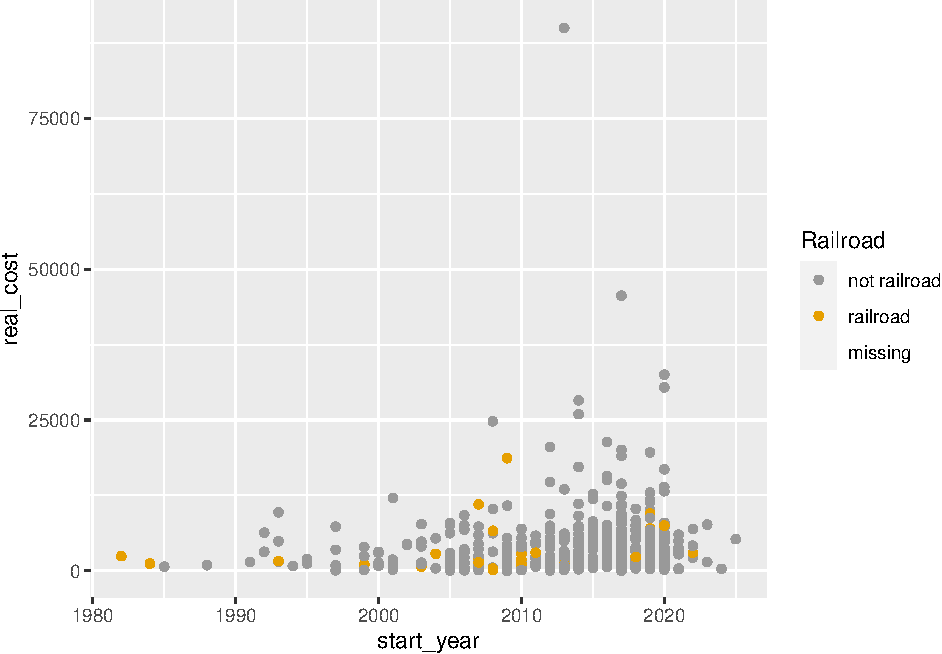
\includegraphics{2021_01_05_tidy_tuesday_files/figure-latex/Visualize-1.pdf}

\begin{Shaded}
\begin{Highlighting}[]
\CommentTok{# non-railroad vs railroad counts}
\KeywordTok{table}\NormalTok{(transit}\OperatorTok{$}\NormalTok{rr)}
\end{Highlighting}
\end{Shaded}

\begin{verbatim}
## 
##   0   1 
## 502  34
\end{verbatim}

\begin{Shaded}
\begin{Highlighting}[]
\CommentTok{# figure out how to replace 'country' with 'region' by using the 'countrycode' package}
\NormalTok{transit }\OperatorTok
\StringTok{  }\KeywordTok{ggplot}\NormalTok{(}\KeywordTok{aes}\NormalTok{(}\DataTypeTok{x =}\NormalTok{ length, }\DataTypeTok{y =}\NormalTok{ real_cost, }\DataTypeTok{color =}\NormalTok{ country)) }\OperatorTok{+}\StringTok{ }
\StringTok{  }\KeywordTok{geom_point}\NormalTok{()}
\end{Highlighting}
\end{Shaded}

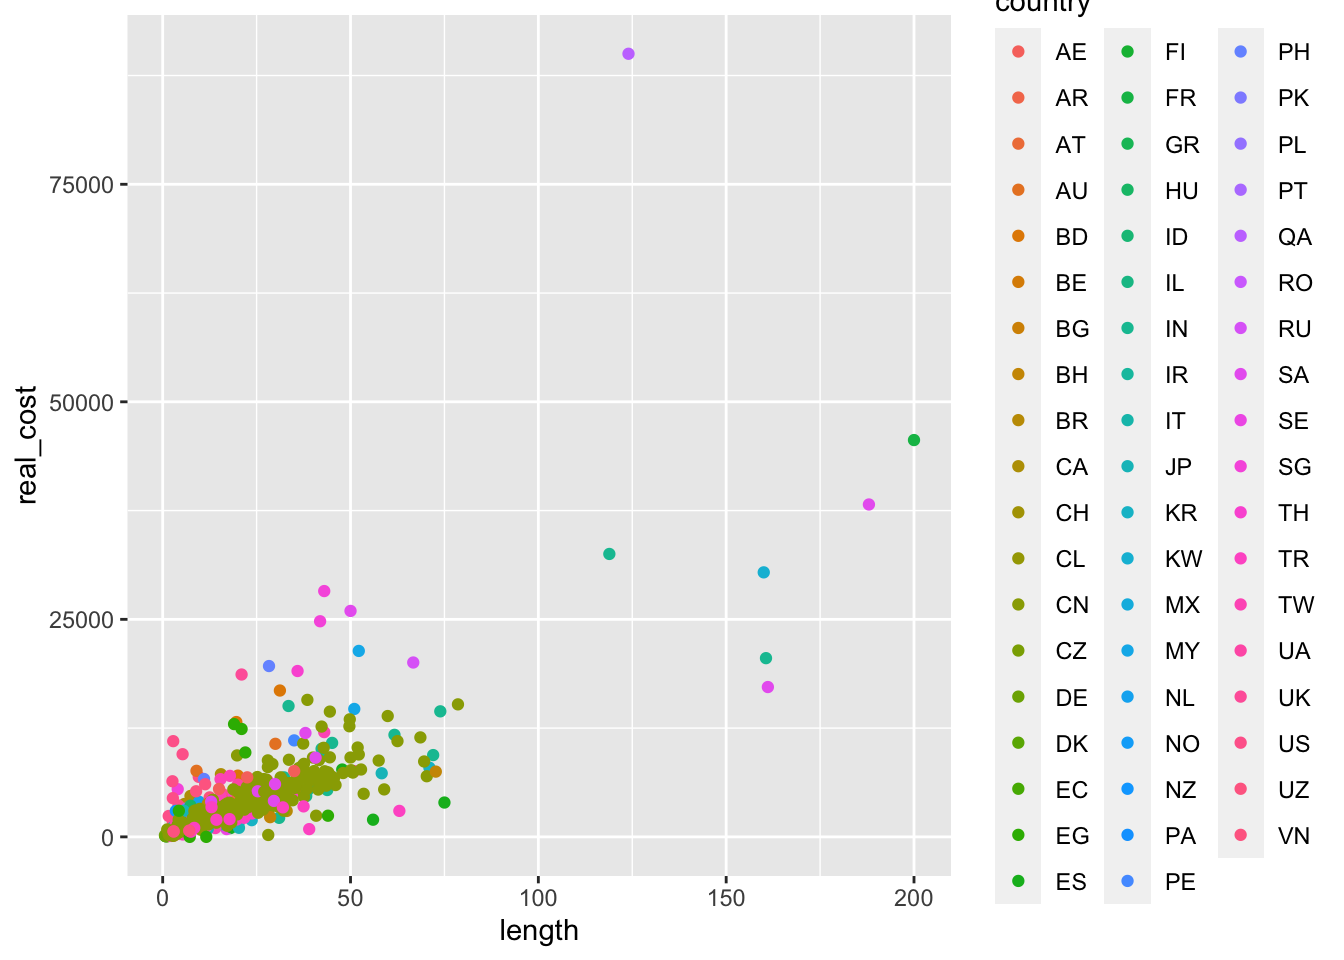
\includegraphics{2021_01_05_tidy_tuesday_files/figure-latex/unnamed-chunk-7-1.pdf}

\begin{Shaded}
\begin{Highlighting}[]
\CommentTok{# run this once we figure out the conuntrycode package!!!}
\CommentTok{#transit %>%}
  \CommentTok{#ggplot(aes(y = real_cost, x = region, color = region)) + }
  \CommentTok{#geom_boxplot() }
\end{Highlighting}
\end{Shaded}

\begin{Shaded}
\begin{Highlighting}[]
\KeywordTok{library}\NormalTok{(knitr)}
\CommentTok{#knit('2021_01_05_tidy_tuesday.Rmd', encoding = 'UTF-8')}
\end{Highlighting}
\end{Shaded}

\end{document}
